\section{Matrix Factorization Visualization}

For each movie \textit{j}, it can be visualized as a 2D vector using the coordinates $\tilde{V}[:,j]$ ($j^{th}$ column of $\tilde{V}$), where $\tilde{V}$ is obtained from the previous section. We show 10 random movies in Figure~\ref{fig:tenRandom}, the most popular 10 movies in Figure~\ref{fig:tenMostPopular} and the best 10 movies in Figure~\ref{fig:tenBest}. In general there is little correlation between distance in the plots and movie similarity as seen by the authors. For example, Scream and Star Wars are very close in Figure~\ref{fig:tenMostPopular} even though the movies do not seem similar. 

We observe that the most popular 10 movies seemed to be divided (into 2 spaces) by the line $y = x$, while the best 10 movies cover the 2D space more uniformly. The reason for this trend is unclear and may be a simple coincidence.  

\begin{figure}[H]
\centering
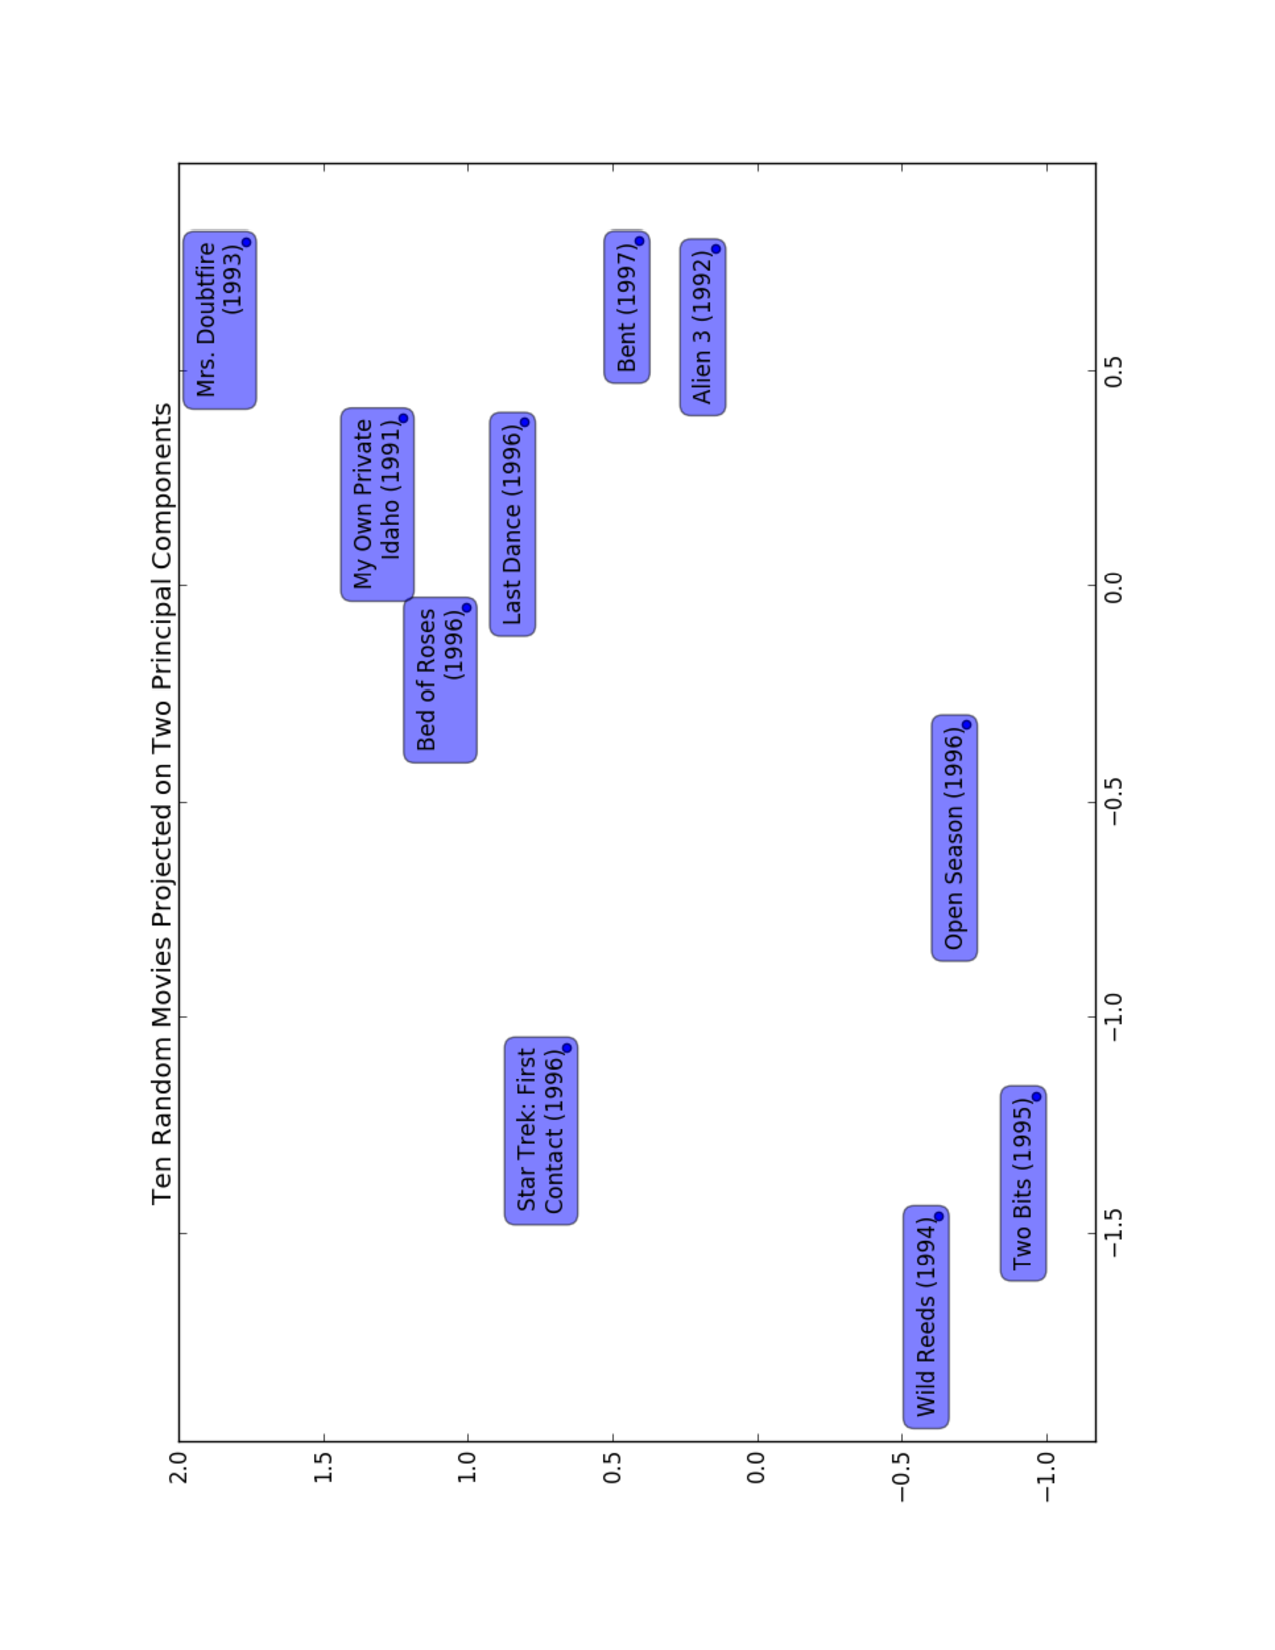
\includegraphics[width=0.75\textwidth, trim = 2cm 2.5cm 2cm 1.8cm, clip=true]{Random_10_Movies.pdf}
 \caption{Ten Random movies projected along two principal components.}
\label{fig:tenRandom}
\end{figure}


\begin{figure}[H]
\centering
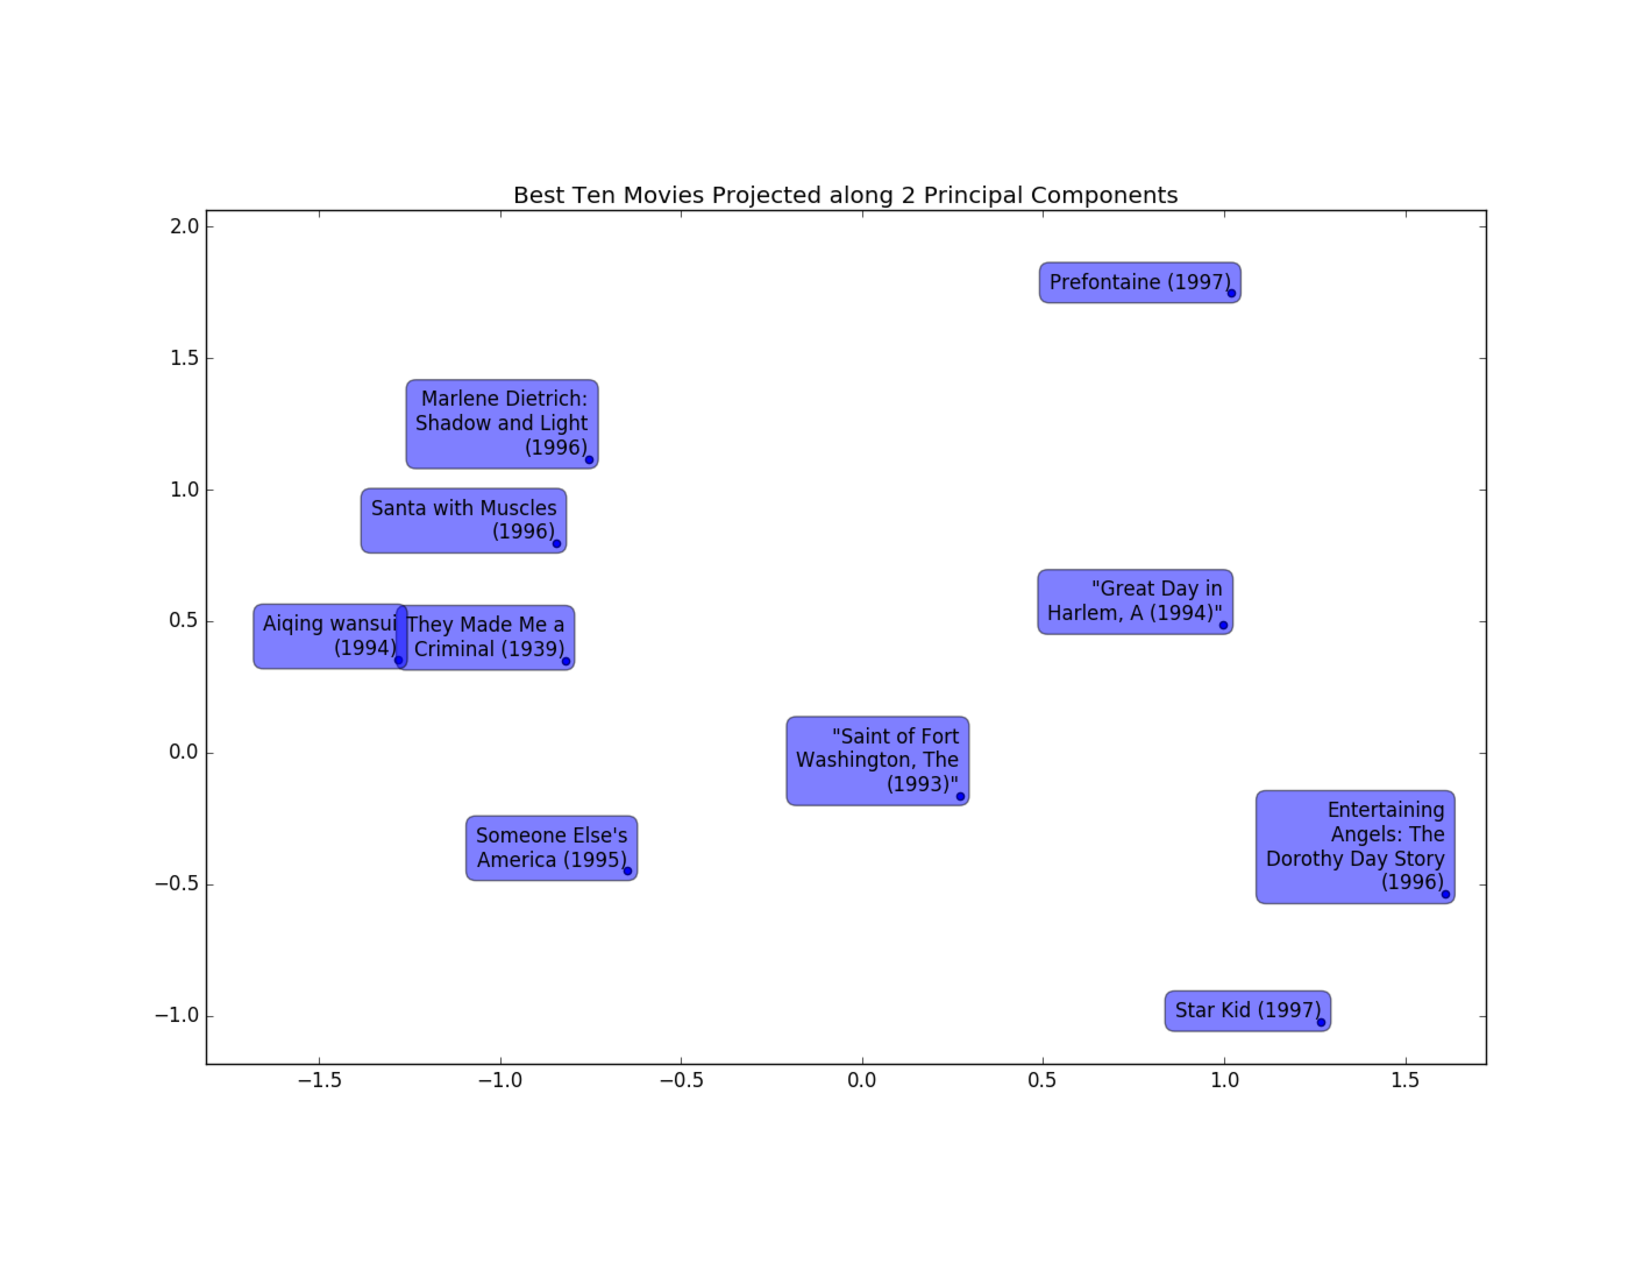
\includegraphics[width=0.75\textwidth, trim = 2cm 2.8cm 2cm 2.5cm, clip=true]{Best_10_Movies.pdf}
 \caption{Best ten movies projected along two principal components.}
\label{fig:tenBest}
\end{figure}


\begin{figure}[H]
\centering
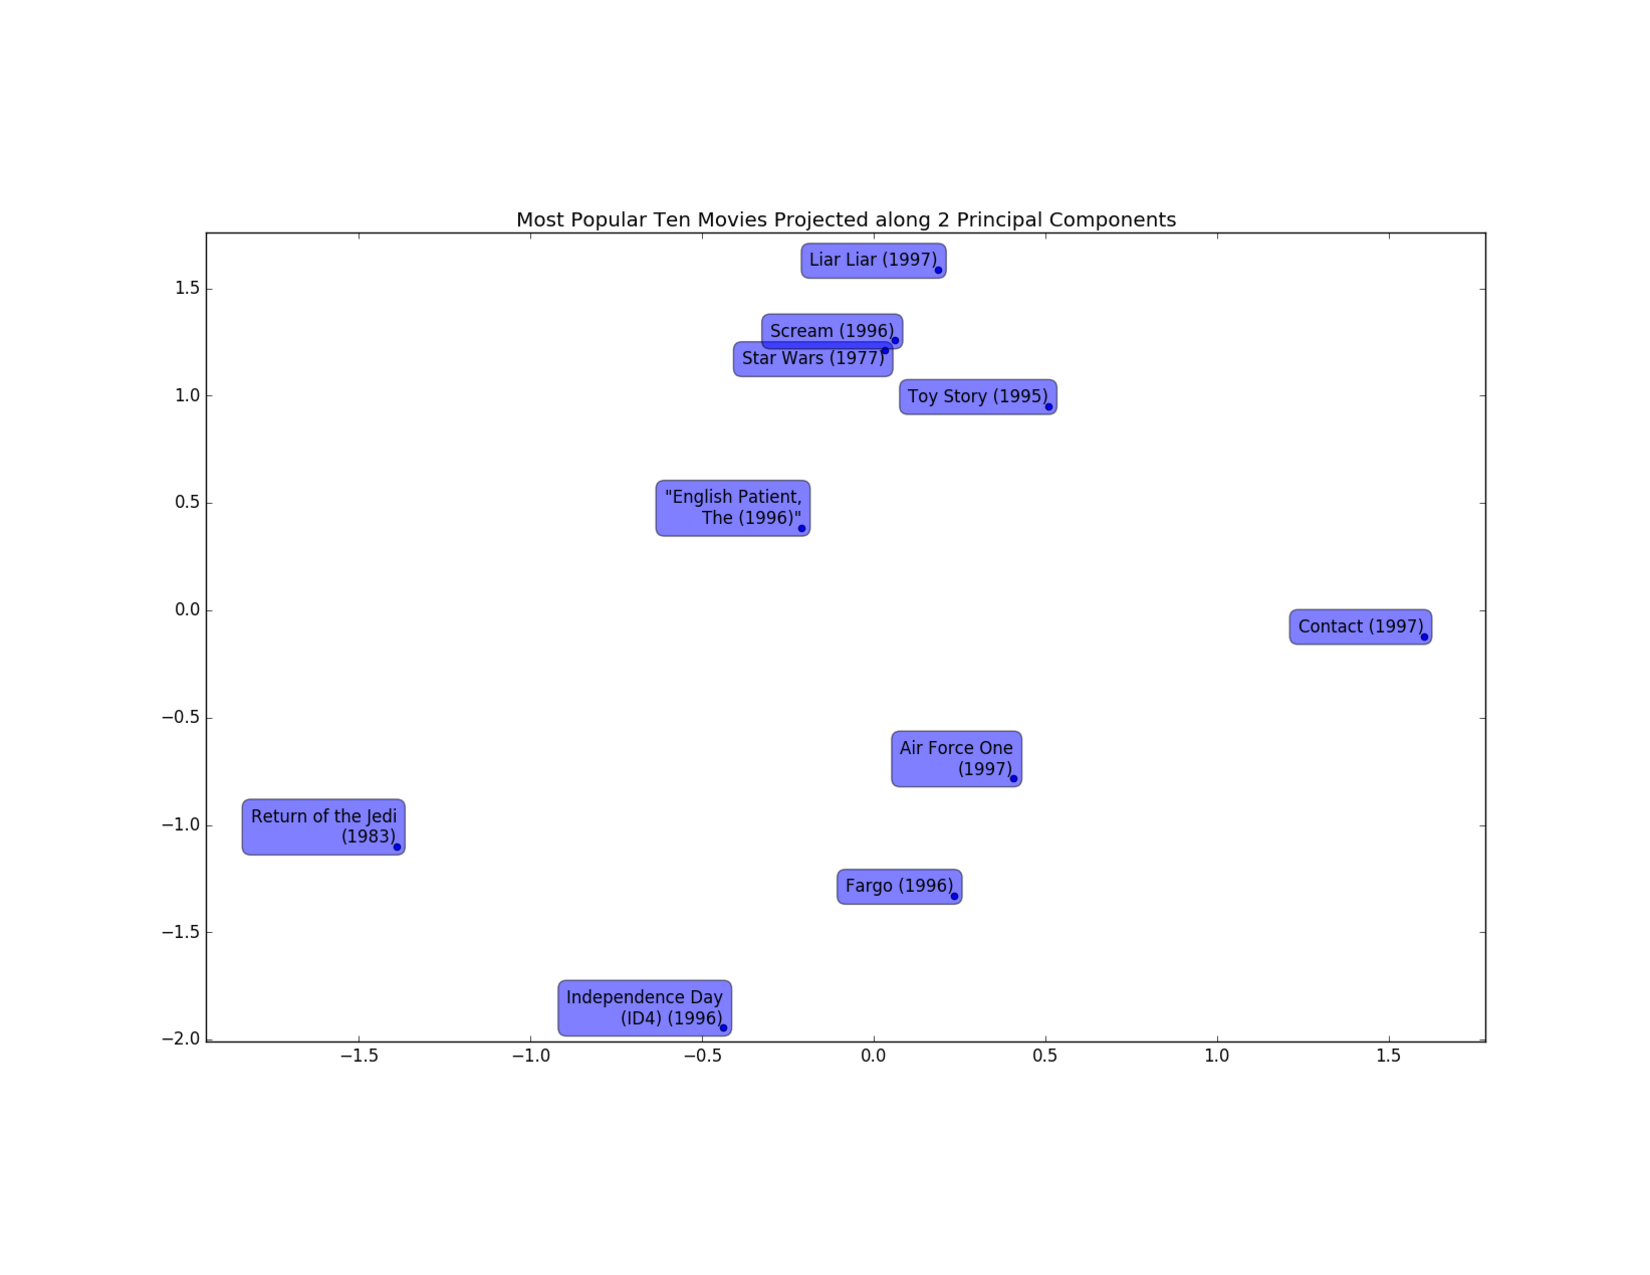
\includegraphics[width=0.9\textwidth, trim = 2cm 2.8cm 2cm 2.5cm, clip=true]{Popular_10_Movies.pdf}
 \caption{Most popular ten movies projected along two principal components.}
\label{fig:tenMostPopular}
\end{figure}

Figure~\ref{fig:tg} shows the representation for 10 random movies within the genres: horror, children and fantasy. The chosen movies within each genre are loosely clustered together, for example horror movies are mostly located on the bottom left corner and fantasy movies on the upper right corner. We can visualize the mean representation with its variance for each genre in Figure~\ref{fig:tgMV}. However, in general, the variance for each given genre is as large as the distance between genre mean centers. Therefore any clustering should be very loose, as observed in the visualization.

\begin{figure}[H]
\centering
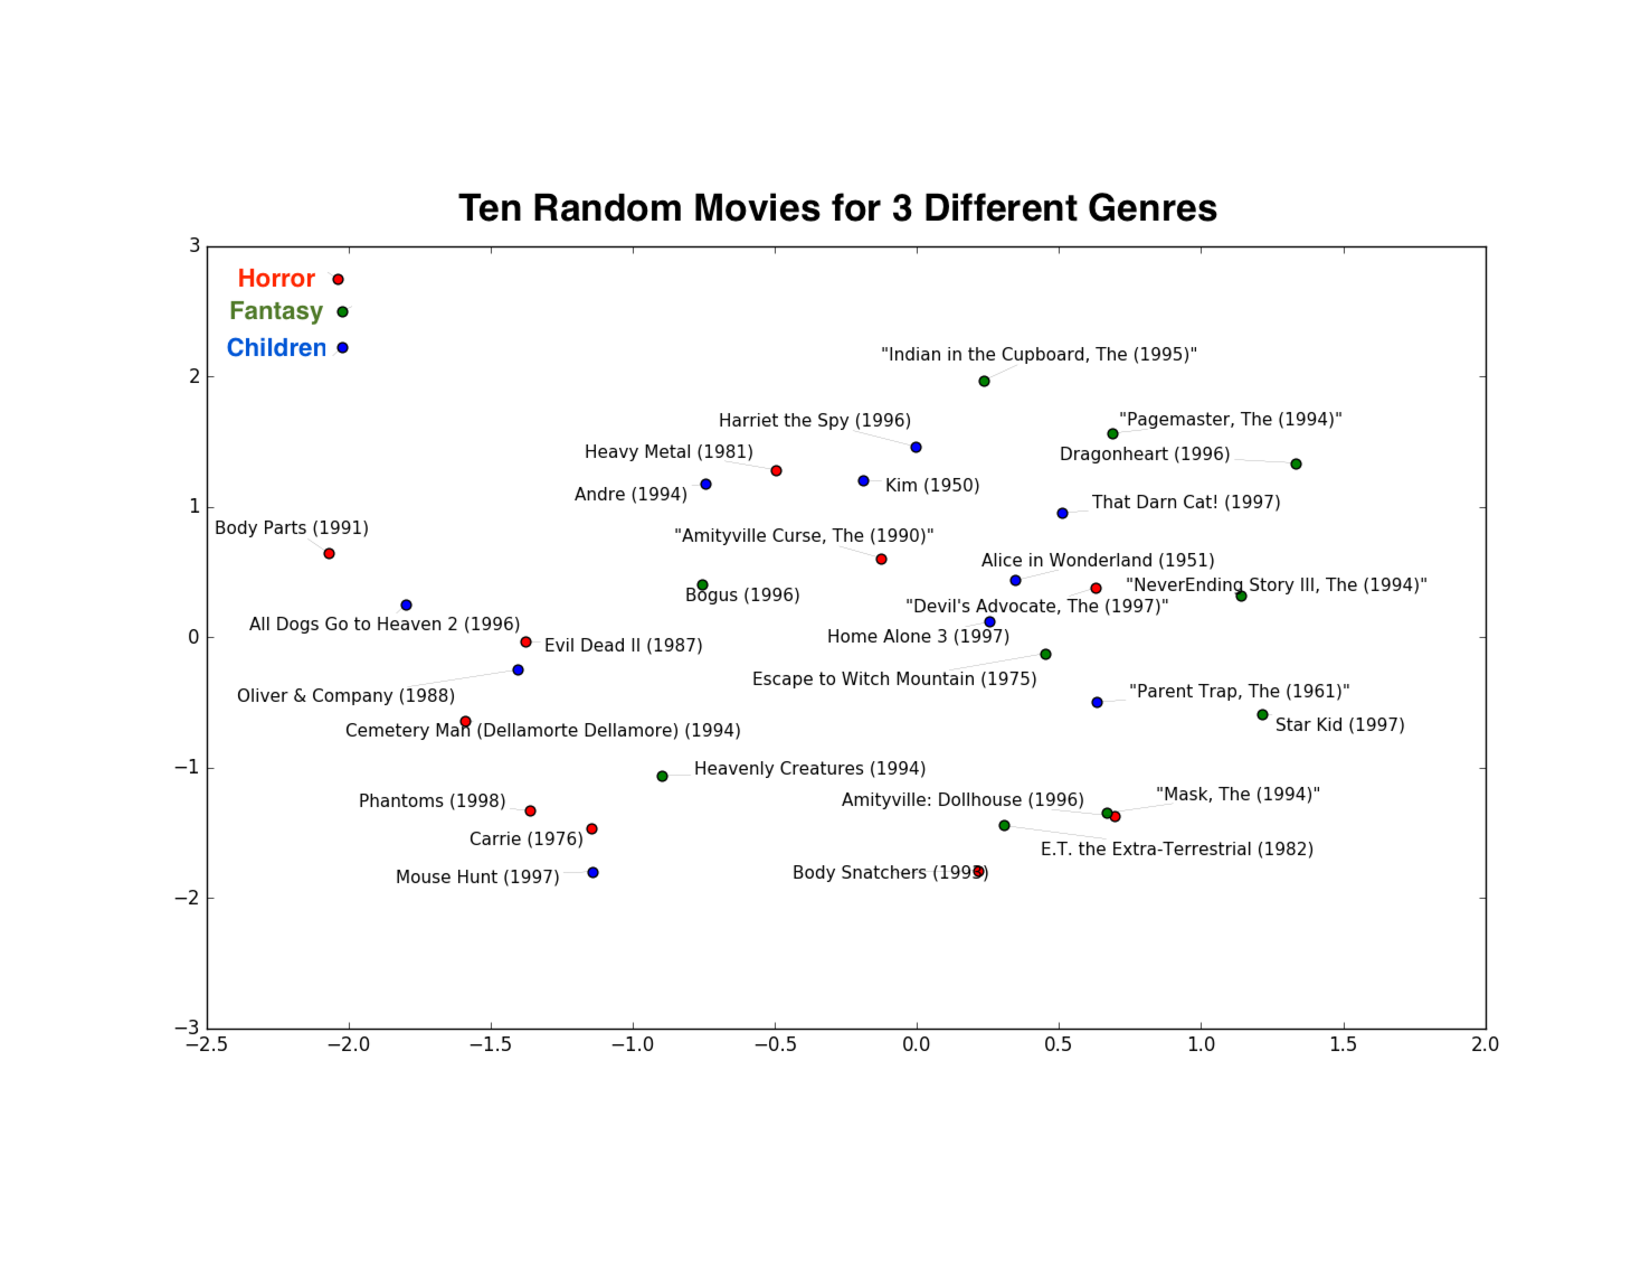
\includegraphics[width=0.85\textwidth, trim = 2cm 3cm 2cm 3cm, clip=true]{Three_Genres.pdf}
 \caption{Ten random movies for the genres horror, fantasy and children. }
\label{fig:tg}
\end{figure}

\begin{figure}[H]
\centering
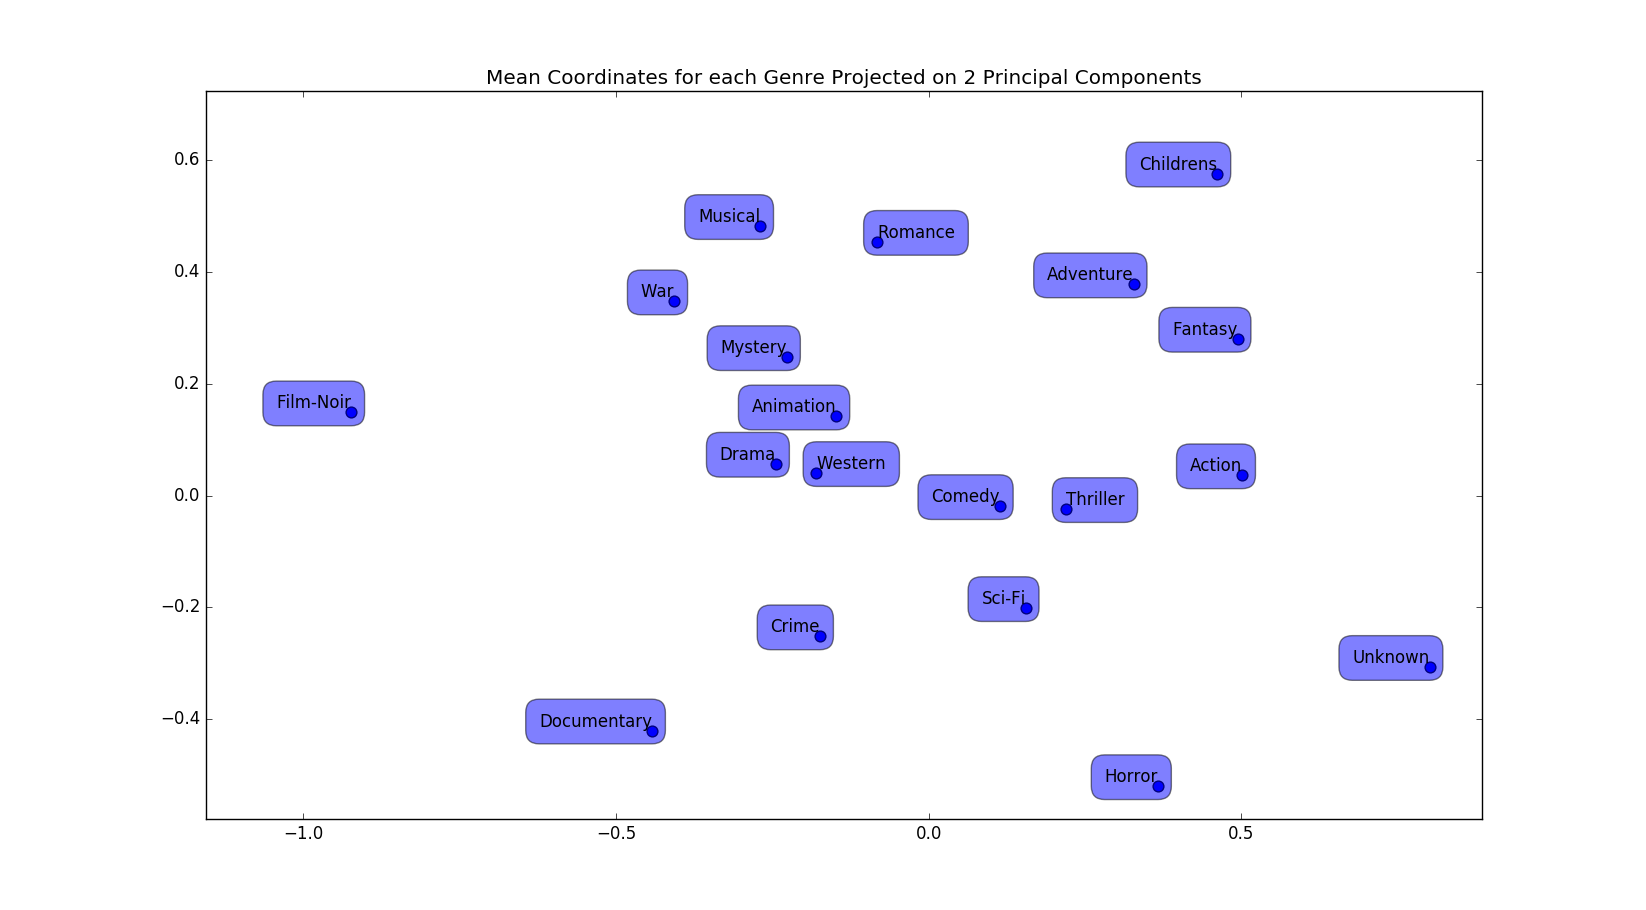
\includegraphics[width=0.9\textwidth, angle =0, trim = 2cm 1cm 2cm 1cm, clip=true]{Mean_Genre.png}
 \caption{Mean Coordinates for each genre with variance.}
\label{fig:tgMeanGenre}
\end{figure}

\begin{figure}[H]
\centering
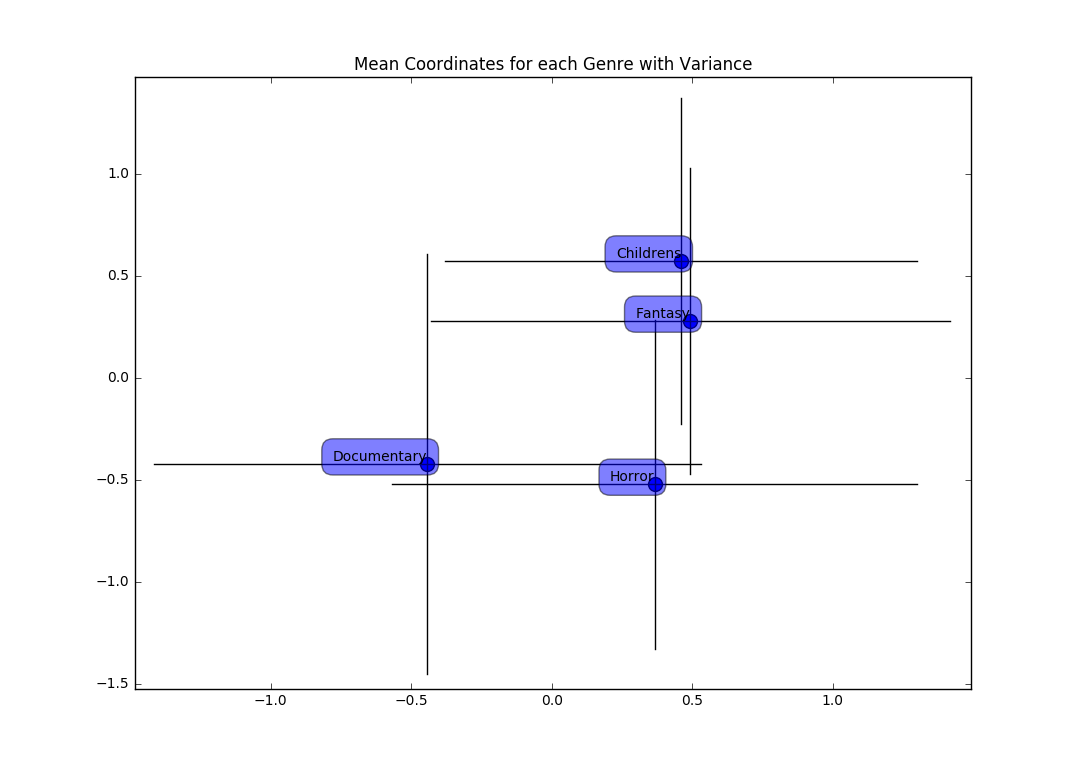
\includegraphics[width=0.7\textwidth, angle =0, trim = 2cm 1cm 2cm 1cm, clip=true]{Mean_Genre_Variance.png}
 \caption{Mean Coordinate with variance for our selection of 3 genres. We also show documentary for reference as a genre far from our selection.}
\label{fig:tgMV}
\end{figure}

Finally, comparing Figure \ref{fig:average-3-genres} and Figure \ref{fig:tgMeanGenre}, we hypothesize that the x axis represents the skewness of the average movie rating distribution. A larger x value implies that the rating distribution skews to the left (i.e. more lower ratings than higher ratings), and a smaller x value implies the opposite. This seems to be a trend within the data. when we look at the rating distribution within each of these genres. 


